\section*{Introduction}

% Introduction
%%     \setlength\itemsep{1em}


In the blockchain ecosystem, coding covers three main aspects:
\begin{enumerate}
    \item \textbf{Development of the blockchain platform}: which is essentially related to the development of the infrastructure (eg, defining new consensus algorithms). During the course, we will not be focusing on this part.
    \item \textbf{Smart contract coding}: which is related to the development of application which runs on blockchain platforms. Although smart contracts can be coded with many different languages, during the course we will be using \textbf{solidity} (de facto standard for ethereum smart contracts)
    \item \textbf{Dapps}: which is related to the development of UI code able to communicate with smart contracts.
\end{enumerate}

%image
\begin{figure}[ht]
    \centering
    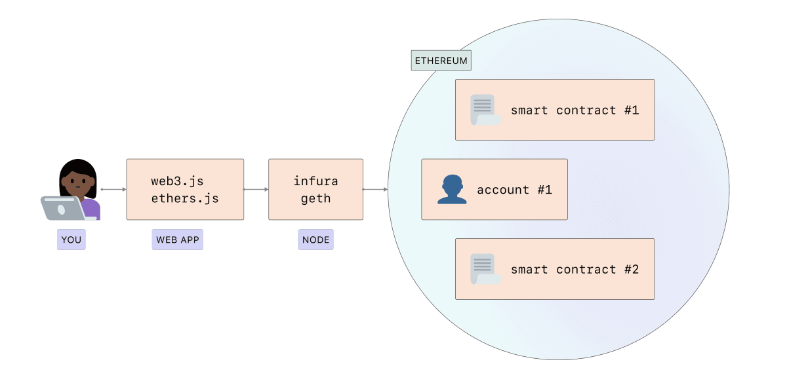
\includegraphics[width=0.75\linewidth]{tikz/appendix - Coding.png}
    \caption{\small A high-level overview of blockchain coding involves users connecting to the blockchain using web3.js. The node utilized is typically an Ethereum node, often implemented through Geth. Additionally, services like Infura offer guidance on setting up nodes within their infrastructure. Within this infrastructure, key elements of the Ethereum node are housed}
    \label{fig:into to blockchain coding}
\end{figure}



The process of developing a blockchain or smart contract typically follows these steps:

\begin{enumerate}
    \item \label{ls: set-blockchian} \textbf{Setting Up the Blockchain}: This step involves to set up the netwrok either in your machine or in cloud and requires:
    
    \begin{itemize}
     \setlength\itemsep{1em}
        \item Choosing Network Type: Determine whether it's a public or private blockchain.
        \item Creating Account with key-pair: an account is just a node. Every time a node is created, it is assigned with a pair of public/private key. Losing these keys results in loss of access.
        \item Installing Ethereum Client: Options include Geth, Besu, etc.
        \item Configuring Client: This involves setting up initial rules for the network, such as consensus algorithm, gas limit, difficulty, etc. Correct configuration is vital to avoid the need for subsequent forks.
        \item Starting Client.
    \end{itemize}
    \item \textbf{Developing Smart Contracts}: Based on the problem to be solved, develop the smart contract.
    \item \textbf{Testing Smart Contracts}: Testing is crucial as smart contracts cannot be modified. In private networks, releasing patches might be possible.
    \item \textbf{Deploying Smart Contracts}: The deployment process requires the use of an account, as it's necessary for deployment.
    \item \textbf{Developing DApps (Decentralized Applications)}:  Interaction with the blockchain occurs through DApps. While wallets like MetaMask enable transactions, they have limited functionalities. ERC-20 tokens can be managed by wallets, but custom UI logic cannot be implemented. DApps serve as the bridge between applications and smart contracts.
    \item \textbf{Deploying DApps}: Deployment methods vary depending on the application type. For web-based applications, providing the IP address is typically necessary.
\end{enumerate}

\subsection{Definitions}

\paragraph{Ethereum client} A client is an implementation of Ethereum that verifies data according to protocol rules and secures the network (eg, Geth). A node must run two clients: a consensus client and an execution client.

The \textbf{execution client} (EL client) listens for new transactions broadcasted on the network, executes them in the EVM, and maintains the latest state and database of all current Ethereum data.

The \textbf{consensus client} (Beacon node, CL client) implements the proof-of-stake consensus algorithm, enabling the network to reach agreement based on data validated by the execution client. Additionally, there is a third piece of software called a "validator" that can be added to the consensus client, allowing the node to participate in securing the network.





\paragraph{Node}
A "node" is any instance of Ethereum client software connected to other computers also running Ethereum software, forming a network. Depending on specific needs, there are three different types of nodes that can be run by any client:

\begin{itemize}
    \item \textbf{Full Node}: This type of node holds a complete copy of the blockchain; it stores and can distribute all data within each block from the Ethereum network. A full node also participates in block validation.
    \item \textbf{Light Node}: Light nodes manage less information. Although they store a complete copy of the blockchain, light nodes only store information about the headers of each block (basic information stored in a block such as a timestamp and the hash of the previous block). They are capable of verifying data validity but do not fully participate in block validation.
    \item \textbf{Archive Node}: Archive nodes are nodes that store all the information of a full node and create an archive of historical states of the blockchain. Archive nodes retain historical data even after a client has finished synchronization.
\end{itemize}

Depending on the node type, there are different synchronization methods: this refers to the speed at which your node is able to retrieve updated information so that your client can interpret it.

\begin{itemize}
    \item \textbf{Full Sync}: downloads all blocks and verifies all transactions
    \item \textbf{Light Sync}: downloads all blocks and verifies just all headers (no transaction)
    \item \textbf{Snap Sync}: starts syncing from some recent blocks (blocks and verifies all transactions of recent transactions)
\end{itemize}

\paragraph{Type of Network} In Ethereum, a network can be either private or public. 

\textbf{Public networks} are accessible to anyone (go to Etherscan). The main public networks in Ethereum include \textit{Mainnet}, \textit{Goerli testnet}, and \textit{Rinkeby testnet}. To interact on these networks, users typically need Ether. However, there are test networks like \textit{falsnet} specifically designed for testing smart contracts and other functionalities without using real Ether.

\textbf{Private networks} or permissioned networks in Ethereum are isolated from the public network and operate independently. They often incorporate specific consensus mechanisms tailored to their needs. Depending on the Ethereum client being used, different consensus mechanisms may be implemented (for example, Geth implements authority consensus).

In private networks, private transactions are implemented differently from public ones. While all transactions in the public Ethereum network occur openly, in private networks, the content of transactions is hashed and included in the main transaction, maintaining privacy.

Two common types of private networks are Development network and Consortium network.

\paragraph{Genesis file}

The Genesis file serves as a configuration file essential for bootstrapping the network, marking the starting point of the blockchain. It defines crucial parameters and initial conditions for the network, including the genesis block, which is the very first block in the blockchain. 

Inside a genesis file, at least the following parameters should be defined:
\begin{itemize}
    \item \textbf{Chain ID}: A unique identifier for the network. On the Ethereum mainnet, this ID is predefined, while for private networks, you define your own.
    \item \textbf{Difficulty}: The initial difficulty level of the network, which dictates the complexity of the proof-of-work algorithm and thereby affects the rate at which new blocks can be mined.
    \item \textbf{Gas Limit}: The maximum amount of gas permitted in a single block. Gas is a measure of computational effort required to execute operations on the Ethereum network, and this limit restricts the number of transactions that can be included in a block.
    \item \textbf{Timestamp}: The timestamp for the first block on the network.
    \item \textbf{Nonce}: A value that is changed repeatedly to create a valid proof-of-work.
    \item \textbf{Allocation}: Specifies the initial distribution of Ether to designated addresses/accounts on the network.
    \item \textbf{Consensus rules}: The rules for validating transactions and adding them to the blockchain.
\end{itemize}

In the following image, we have provided an example:

\begin{figure}[ht]
    \centering
    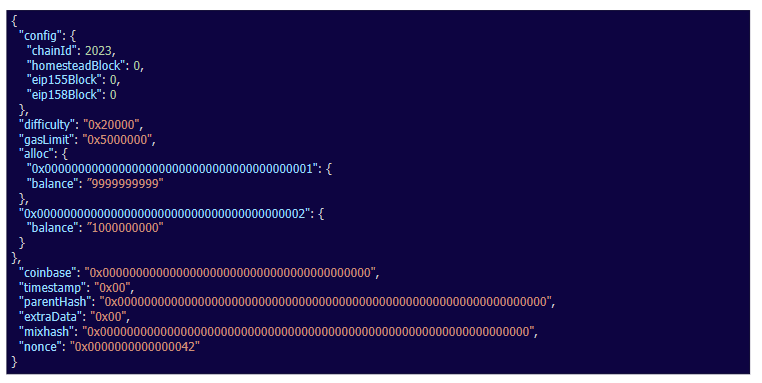
\includegraphics[width=0.75\linewidth]{tikz/appendix - Genesis File.png}
    \caption{Example of a genesis file}
    \label{fig:genesis-file}
\end{figure}

In "config" we specify the initial configurations: \textbf{Chain ID} Identifies the chain; \textbf{Homestead Block} refers to the Ethereum Homestead release, denoted by '0' to signify its usage;\textbf{EIP-155 Block} represents Ethereum Improvement Proposals, fostering developer contributions for Ethereum's enhancement.

Othe parameters are \textbf{difficulty}, \textbf{Gas Limit}, \textbf{alloc} which specifies pre-funds addresses, each specified as a 40-digit hexadecimal string (160 bit), and \textbf{ExtraData} that contains parameters linking to the consensus mechanism; currently unspecified.


\section{Setting up a Private Network}

To establish a blockchain network (point \ref{fig:into to blockchain coding} ), the following elements are necessary:

\begin{itemize}
    \item Network: meaning the blockchain netwrok should be installed in your machine
    \item Node: meaning setting up the nodes participant in your network
    \item Bootnode
    \item Miners
    \item Accounts: holds keys for interacting with the network
    \item Genesis file
\end{itemize}



